\begin{sloppypar*}
    Whereas, previous work in this field has focused on either the embedding
    generation algorithm or on a particular modality that such an algorithm can
    accept, in this research, the authors attempt to compare the effect of
    \textbf{different data modalities} for generating \textbf{functional gene
    embeddings} on a set of downstream tasks such as `\textit{predict disease-gene
    list}', `\textit{predict cancer drivers}', `\textit{predict phenotype-gene
    associations}' and `\textit{predict scores from genome-wide studies}'. \hfill \break

    \noindent The two overall objectives were:
    \begin{enumerate}
        \item generate embeddings from various modalities
        \item ensure that the embeddings are free from bias
    \end{enumerate}
    
    \noindent The various modalities utilized are - `\textbf{quantitative OMICS}', 
    `\textbf{protein-protein interaction networks}' and `\textbf{literature}'. The 
    authors have observed that there is no clear winner for the data source/type
    and in general there is a dependance on the particular downstream task. Further,
    they have also observed the problem of undercoverage bias in gene embeddings
    generated from literature. Figure \ref{fig:mindmap} provides an overview of
    this paper.

    \begin{figure}
        \centering
        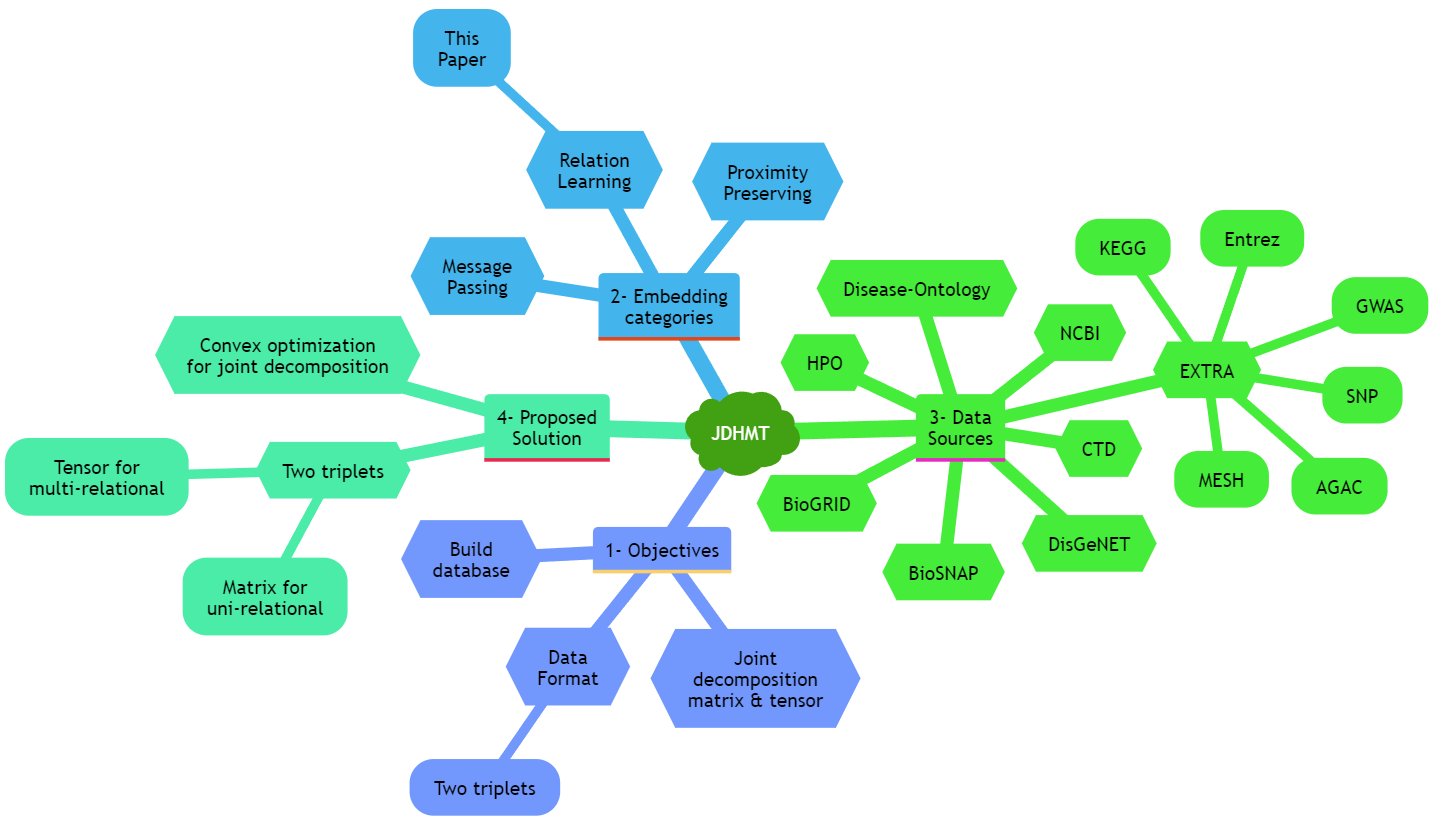
\includegraphics[width=170mm,scale=1]{mindmap.png}
        \caption{Mindmap}
        \label{fig:mindmap}
    \end{figure}
\end{sloppypar*}